\documentclass[
	letterpaper, % Paper size, specify a4paper (A4) or letterpaper (US letter)
	10pt, % Default font size, specify 10pt, 11pt or 12pt
]{CSUniSchoolLabReport}

%----------------------------------------------------------------------------------------
%	REPORT INFORMATION
%----------------------------------------------------------------------------------------

\title{Lab Three\\ Fundamentals of Electronics \\ EECE2412/3} % Report title

\author{Michael \textsc{Brodskiy}\\ \small \href{mailto:Brodskiy.M@Northeastern.edu}{Brodskiy.M@Northeastern.edu}}

\date{October 29, 2024} % Date of the report

%----------------------------------------------------------------------------------------


\begin{document}

\maketitle % Insert the title, author and date using the information specified above

\begin{center}
	\begin{tabular}{l r}
		Date Performed: & October 15/22, 2024 \\ % Date the experiment was performed
        Partner: & Rahul \textsc{Singh} \\ % Partner names
		Instructor: & Professor \textsc{Onabajo} \\ % Instructor/supervisor
        TAs: & Ming \textsc{Xiang} \& Amr \textsc{Kassab} \\ % Teachers Assistants 
	\end{tabular}
\end{center}

\newpage

\begin{abstract}

  The goal of this laboratory experiment is to orient the performing individual with bipolar junction transistors (BJTs). Common regions (active, saturated, and cut-off) are explored, in addition to the effects of temperature variance on BJT performance. Finally, a light-emitting diode (LED) light-sensing circuit is constructed with a photocell. 

\end{abstract}

\begin{flushleft}

  \textsc{Keywords:} \underline{BJT}, \underline{active}, \underline{saturated}, \underline{cut-off}, \underline{temperature variance}, \underline{LED}, \underline{photocell}

\end{flushleft}

\newpage

\tableofcontents
\listoffigures

\newpage

\section{Equipment}

Available equipment included:\\

\begin{itemize}

  \item 2N3904 Bipolar Junction Transistors

  \item Light-Emitting Diodes (varying colors)

  \item Basic Circuit Components (Wires, Inductors, Capacitors, etc.)

  \item Keysight EDU36311A Dual DC Power Supply

  \item Photocell (Light-Varying Resistor)

\end{itemize}

\newpage

\section{Experimental Procedure}

We begin by constructing the following circuit:

\begin{figure}[H]
  \centering
  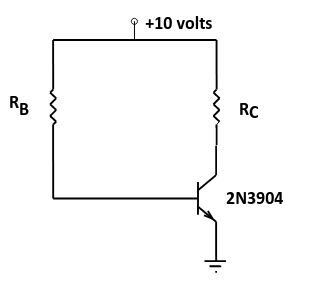
\includegraphics[width=.7\textwidth]{Figures/L3F1}
  \caption{BJT Biasing Circuit}
  \label{fig:1}
\end{figure}

We proceed to test various configurations which place the 2N3904 in common regions, such as active, saturated, and cut-off.

\subsection{The Forward-Active Region (with varying $\beta$)}

Using the circuit shown in Figure \ref{fig:1}, with $R_B=316.7[\si{\kilo\ohm}]$ and $R_C=1.003[\si{\kilo\ohm}]$, we place the BJT into its active region (supporting calculations are present in the pre-lab). Measuring $V_{CE}$ and $V_{BE}$ for both of our BJTs, we find:

$$V_{BE_1}=.708[\si{\volt}]\quad\text{ and }\quad V_{CE_1}=3.394[\si{\volt}]$$
$$V_{BE_2}=.704[\si{\volt}]\quad\text{ and }\quad V_{CE_2}=3.378[\si{\volt}]$$

We know the BJT is in its active region since, based on the above measurements, $V_{CE}>V_{BE}$ (or, alternatively $V_{BE}>0$ and $V_{BC}<0$).

Using the data from above, we may calculate $I_B$, $I_C$, and $\beta$:

$$I_{B_1}=\frac{10-.708}{316.7k}\quad\text{ and }\quad I_{C_1}=\frac{10-3.394}{1003}$$
$$\boxed{I_{B_1}=29.34[\si{\micro\ampere}]\quad\text{ and }\quad I_{C_1}=6.586[\si{\milli\ampere}]}$$

$$I_{B_2}=\frac{10-.704}{316.7k}\quad\text{ and }\quad I_{C_1}=\frac{10-3.378}{1003}$$
$$\boxed{I_{B_1}=29.353[\si{\micro\ampere}]\quad\text{ and }\quad I_{C_1}=6.6022[\si{\milli\ampere}]}$$

From this, we find the direct current (DC) gains:

$$\beta_1=\frac{6.586}{.02934}$$
$$\boxed{\beta_1=224.47}$$

$$\beta_2=\frac{6.6022}{.029353}$$
$$\boxed{\beta_2=224.92}$$

\subsubsection{Using Curve Tracers}

Per the curve tracer presented in class, we would expect $I_B=40[\si{\micro\ampere}]$ for our $I_C$ value. This gives us a $\beta$ of:

$$\beta_{curve}=\frac{6}{.04}$$
$$\boxed{\beta_{curve}=150}$$

\subsubsection{Tolerance and Standard Deviation of Gain}

It would be difficult to design a circuit with $\beta=150\pm 1\%$ because, even within the same model of BJT, there is much variation; however, it should still be practical to meet this strict tolerance. This is further supported by the variance of $\beta$ presented in the BJT data sheets attached to the laboratory experiment. Though the tested transistors are all within specification, there is a great amount of variance, which we can calculate using the standard deviation. We obtain two of each $\beta$ value from other groups:

$$\beta_1=186,196$$
$$\beta_2=201,217$$

The average of the gains is:

$$\beta_1^{avg}=202.16$$
$$\beta_2^{avg}=214.31$$

Thus, we get standard deviations of:

$$\boxed{\sigma_{\beta_1}=19.96\quad\text{ and }\sigma_{\beta_2}=12.185}$$

We may see that these standard deviations are all, more or less, within $1\%$ (for $\beta_1$ it is above for two of the three values), and, therefore, we should be able to design for such a tolerance.

\subsubsection{Thermal Response}

Using a can of refrigerant, we obtain new values:

$$V_{CE}=3.78[\si{\volt}]\quad\text{ and }\quad V_{BE}=.725[\si{\volt}]$$

This gives us:

$$\beta=\frac{\left( \frac{10-3.78}{1003} \right)}{\left( \frac{10-.725}{316700} \right)}$$
$$\boxed{\beta_{cold}=211.48}$$

Per the data sheets, we would expect a drop in $I_C$, which would result in a decrease in $\beta$, as shown above. This would be unwanted in a car stereo system, as colder weather would mean that the amplification would not be as great, thus causing lower volumes.

\subsection{BJT Saturation}

As per the pre-lab, we know that $R_B\leq 208.66[\si{\kilo\ohm}]$ will saturate the BJT. Thus, we select the closest available value: $R_B=157[\si{\kilo\ohm}]$. Measuring the saturation values, we find:

$$V_{CE_1}^{sat}=45[\si{\milli\volt}]\quad\text{ and }\quad V_{BE_1}^{sat}=.906[\si{\volt}]$$
$$V_{CE_2}^{sat}=51.5[\si{\milli\volt}]\quad\text{ and }\quad V_{BE_1}^{sat}=.94[\si{\volt}]$$

We see that there is a lot of variation between even the same model of BJT, and, thus, it is necessary to account for BJT-to-BJT variation. We may find the $\beta$ values for this region:

$$I_{B_1}=\frac{10-.906}{157000}\quad\text{ and }\quad I_{C_1}=\frac{10-.045}{1003}$$
$$\boxed{I_{B_1}=57.92[\si{\micro\ampere}]\quad\text{ and }\quad I_{C_1}=9.925[\si{\milli\ampere}]}$$

$$I_{B_2}=\frac{10-.94}{157000}\quad\text{ and }\quad I_{C_2}=\frac{10-.0515}{1003}$$
$$\boxed{I_{B_1}=57.7[\si{\micro\ampere}]\quad\text{ and }\quad I_{C_1}=9.9187[\si{\milli\ampere}]}$$

This gives us:

$$\beta_1=\frac{9.925}{.05792}$$
$$\boxed{\beta_1=171.36}$$

$$\beta_2=\frac{9.9187}{.0577}$$
$$\boxed{\beta_2=171.90}$$

From this, we see that, if a high $\beta$ is important in a circuit, we want to operate in the active, and not in the saturated region.

\subsection{BJT Cut-Off}

Using the different methods provided, we obtain:

$$V_{CE_1}=10[\si{\volt}]$$
$$V_{CE_2}=9.638[\si{\volt}]$$
$$V_{CE_3}=4.572[\si{\volt}]\quad\text{ (when $R=470[\si{\ohm}]$)}$$

\subsection{BJT Touch-Sensitive Switch}

We may create a touch-activated LED circuit by integrating an LED and replaced $R_B$ with ``touch points'' as show in Figure \ref{fig:2} below:

\begin{figure}[H]
  \centering
  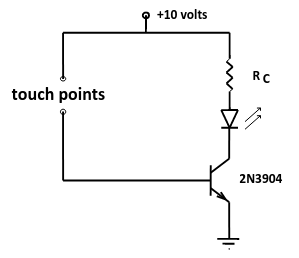
\includegraphics[width=.7\textwidth]{Figures/L3F2}
  \caption{Touch-Activated Circuit}
  \label{fig:2}
\end{figure}

We may thus equate the initial resistance to the resistance of the finger, and call it $R_f$. We now perform all of the necessary BJT calculations:

$$V_{CE}=7.549[\si{\volt}]\quad\text{ and }\quad V_{BE}=.653[\si{\volt}]$$
$$V_{LED}=1.76[\si{\volt}]\quad\text{ and }\quad V_{R_C}=.49[\si{\volt}]$$

The measured values allow us to obtain:

$$\boxed{I_C=\frac{.49}{1003}=.48853[\si{\milli\ampere}]}$$

We can then write:

$$.653=\frac{R_f}{R_f+1003}$$
$$.347R_f=653$$
$$\boxed{R_f=1.882[\si{\mega\ohm}]}$$

From here, we can get:

$$I_B=\frac{.653}{1.882\cdot10^6}$$
$$\boxed{I_B=.34697[\si{\micro\ampere}]}$$

We may observe that, for the circuit without the BJT, the LED would not light up. This is due to the fact that the BJT provides the amplification, which allows the LED to light up, whereas the circuit without the transistor would have very little current, and, therefore, the LED would not turn on.

\subsection{Automatic Night Light}

In this section, we construct two night light circuits: one with immediate response, and one with a one second time delay. First, we measure the resistance of the photocell:

$$\boxed{R_{light}=5.9[\si{\kilo\ohm}]\quad\text{ and }\quad R_{dark}=51[\si{\kilo\ohm}]}$$

The constructed circuit may be seen below:

\begin{figure}[H]
  \centering
  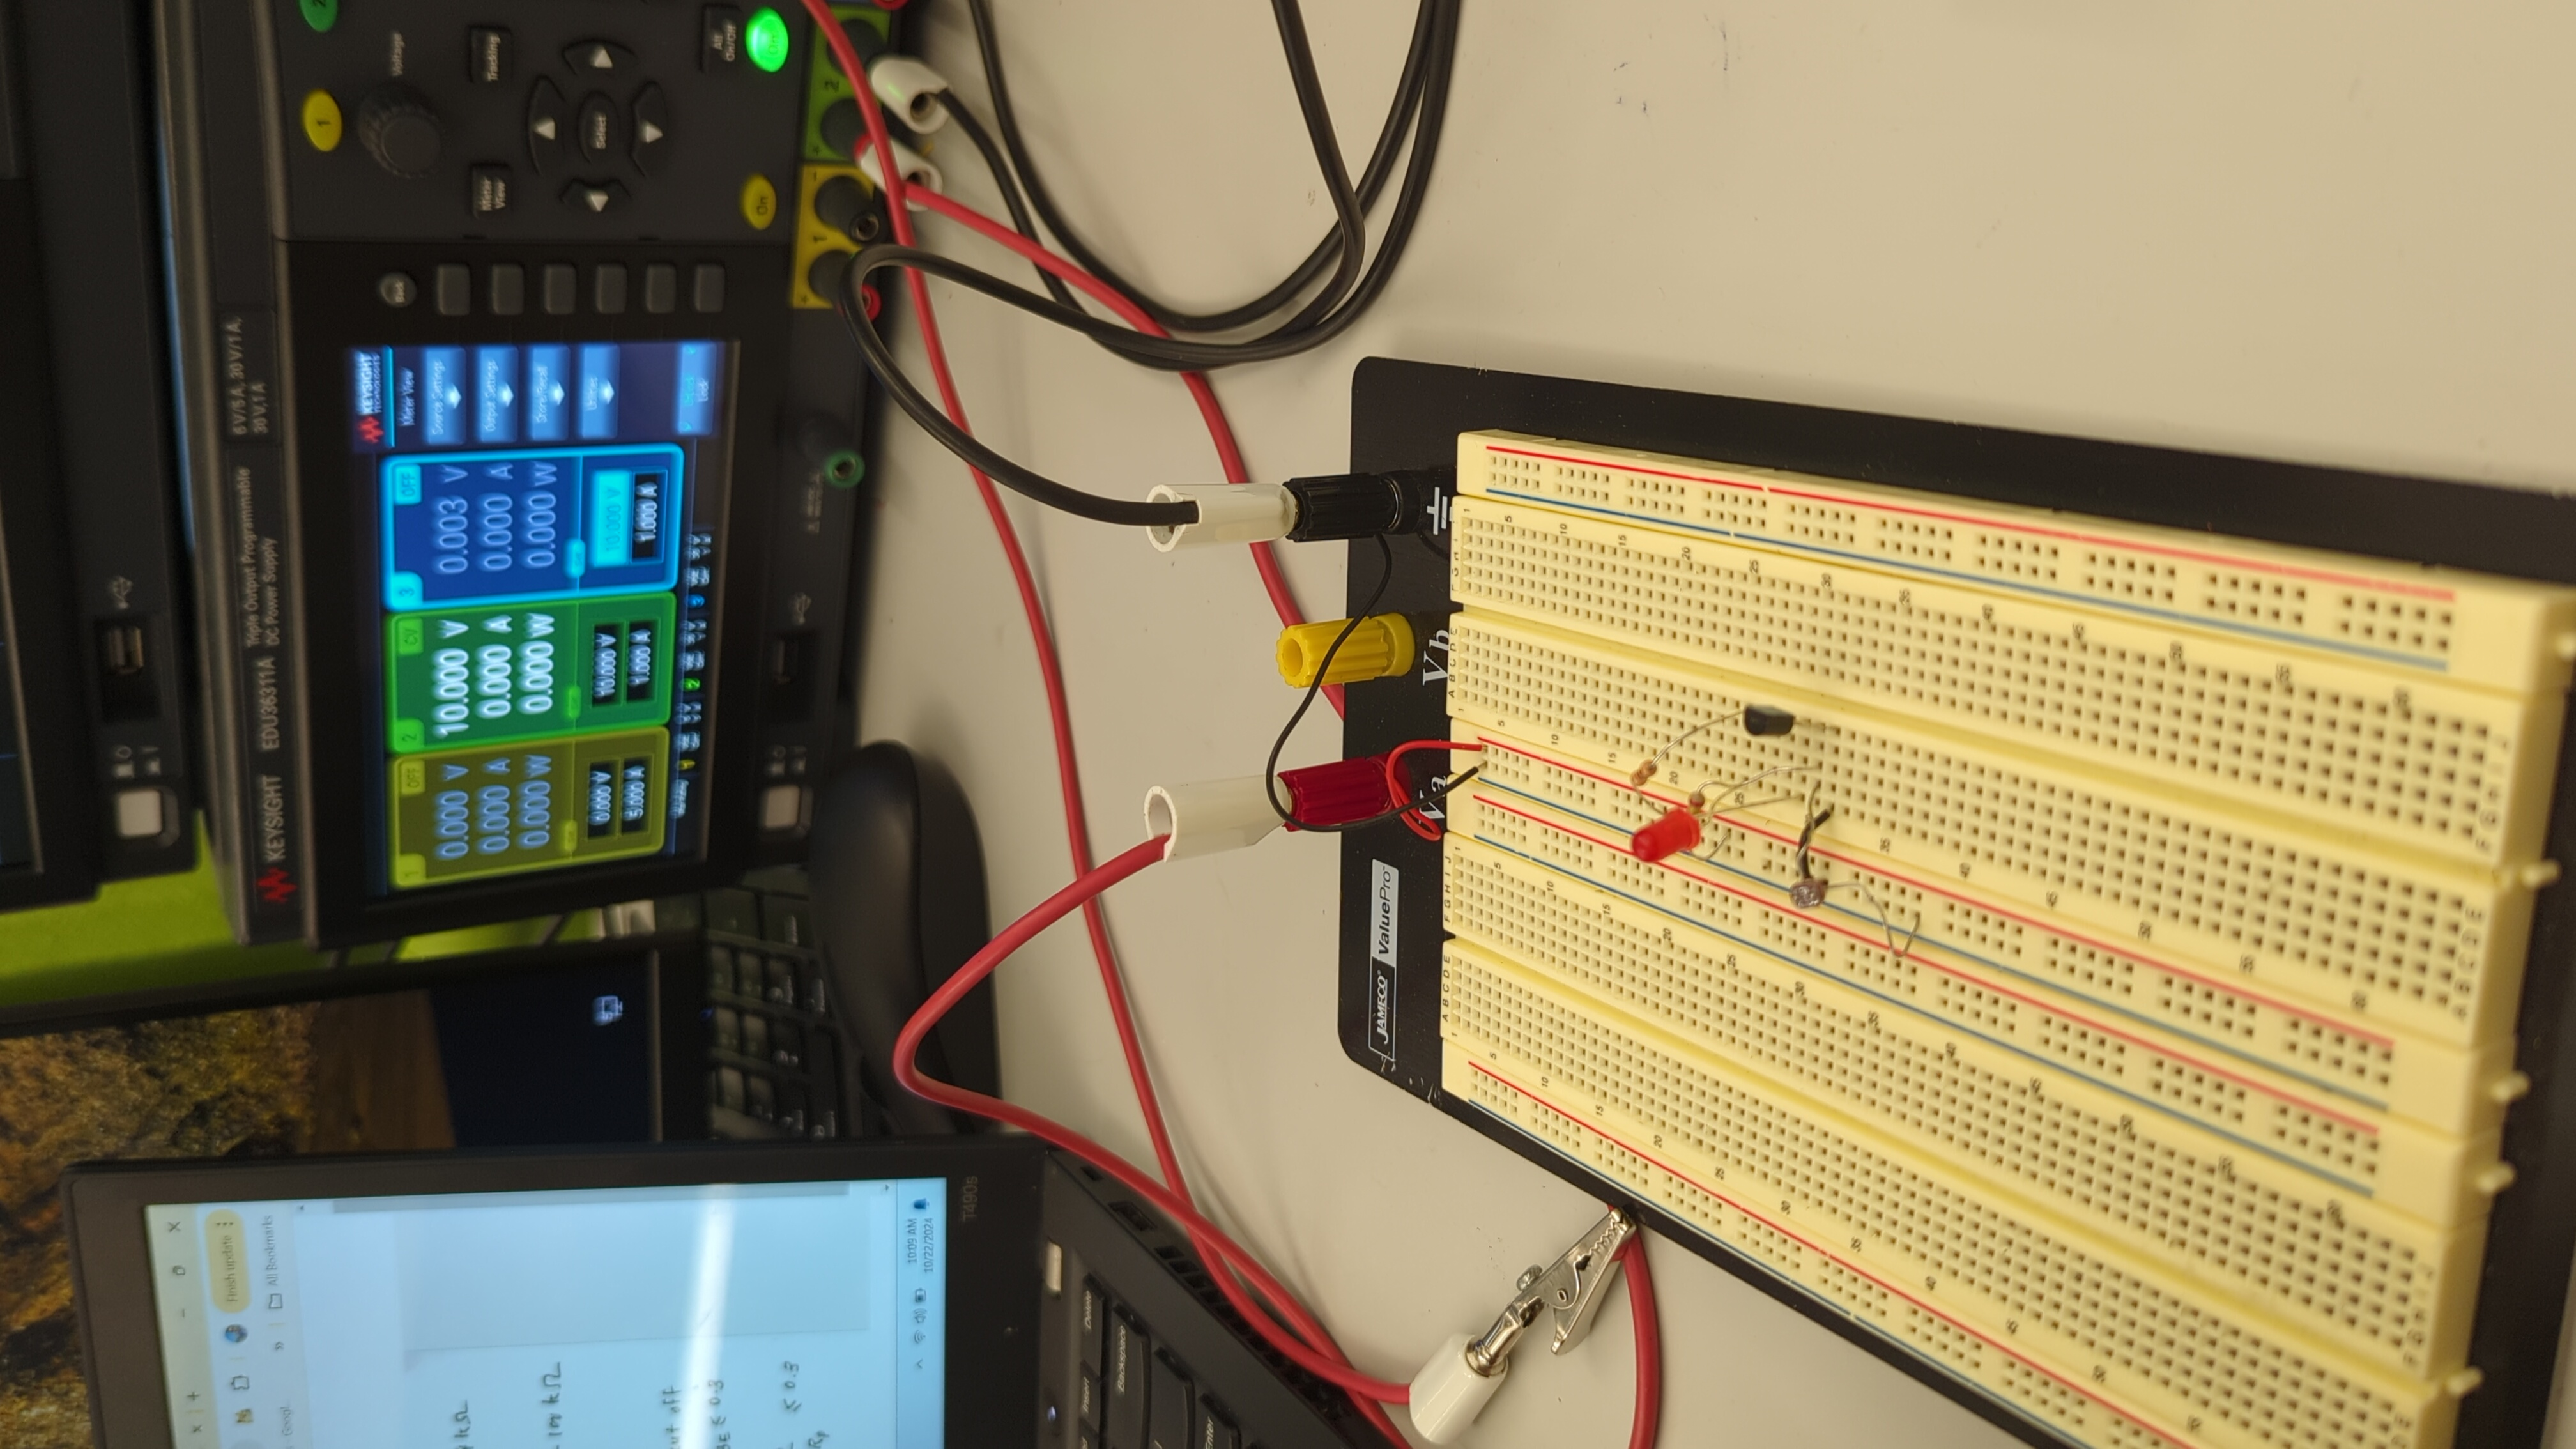
\includegraphics[height=.9\textwidth,angle=270]{Figures/L3C1}
  \caption{Night Light BJT Circuit}
  \label{fig:3}
\end{figure}

The immediate response circuit may be seen below:

\begin{figure}[H]
  \centering
  
\includegraphics[width=.4\textwidth]{Figures/L3Q1}
  \caption{Scan to See Response (or \href{http://Michael.Brodskiy.com/NightLight1.mp4}{click here})}
  \label{fig:4}
\end{figure}

The circuit was then reconstructed with a $1[\si{\milli\farad}]$ capacitor in parallel with the photocell to ensure a time-delayed response. The circuit is shown below:

\begin{figure}[H]
  \centering
  \tikzset{every picture/.style={line width=0.75pt}} %set default line width to 0.75pt        

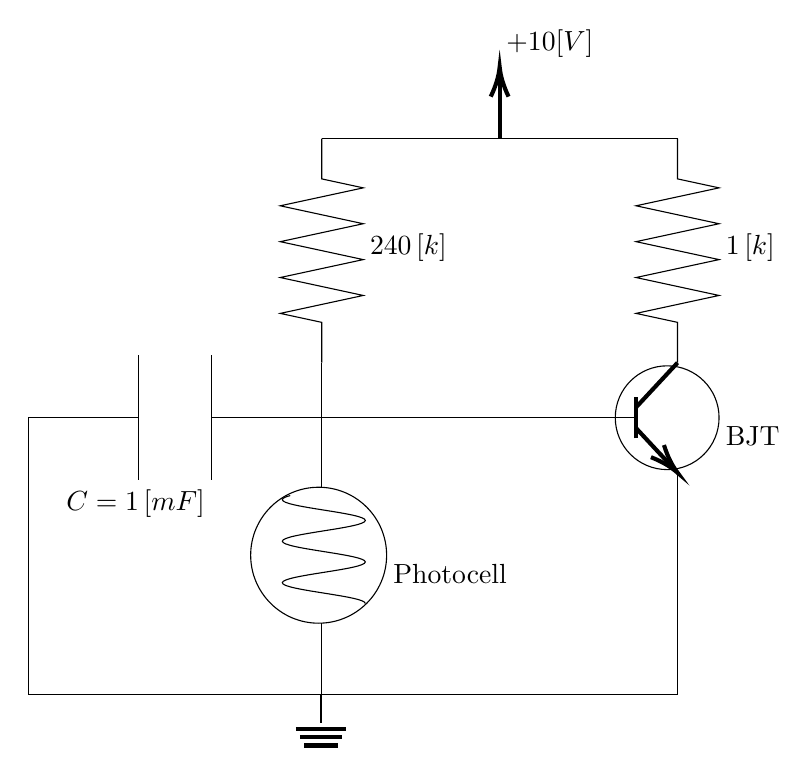
\begin{tikzpicture}[x=0.75pt,y=0.75pt,yscale=-1,xscale=1]
%uncomment if require: \path (0,497); %set diagram left start at 0, and has height of 497

%Shape: Resistor [id:dp08557489822351128] 
\draw   (214,71) -- (214,90.44) -- (234,94.76) -- (194,103.4) -- (234,112.04) -- (194,120.68) -- (234,129.32) -- (194,137.96) -- (234,146.6) -- (194,155.24) -- (214,159.56) -- (214,179) ;
%Straight Lines [id:da10613850567534644] 
\draw    (355.42,205.5) -- (214,205.5) ;
%Shape: Resistor [id:dp42863709400980965] 
\draw   (385.42,71) -- (385.42,90.44) -- (405.42,94.76) -- (365.42,103.4) -- (405.42,112.04) -- (365.42,120.68) -- (405.42,129.32) -- (365.42,137.96) -- (405.42,146.6) -- (365.42,155.24) -- (385.42,159.56) -- (385.42,179) ;
%Shape: Circle [id:dp6263492261348075] 
\draw   (355.42,205.5) .. controls (355.42,191.69) and (366.61,180.5) .. (380.42,180.5) .. controls (394.23,180.5) and (405.42,191.69) .. (405.42,205.5) .. controls (405.42,219.31) and (394.23,230.5) .. (380.42,230.5) .. controls (366.61,230.5) and (355.42,219.31) .. (355.42,205.5) -- cycle ;
%Straight Lines [id:da5434466420085665] 
\draw    (365.42,205.5) -- (355.42,205.5) ;
%Straight Lines [id:da8222789328378522] 
\draw [line width=1.5]    (365.42,215.5) -- (365.42,195.5) ;
%Straight Lines [id:da6868248647799469] 
\draw [line width=1.5]    (365.42,210.5) -- (383.38,229.8) ;
\draw [shift={(385.42,232)}, rotate = 227.07] [color={rgb, 255:red, 0; green, 0; blue, 0 }  ][line width=1.5]    (14.21,-4.28) .. controls (9.04,-1.82) and (4.3,-0.39) .. (0,0) .. controls (4.3,0.39) and (9.04,1.82) .. (14.21,4.28)   ;
%Straight Lines [id:da7170401481045089] 
\draw [line width=1.5]    (385.42,179) -- (365.42,200.5) ;
%Straight Lines [id:da09379764529365986] 
\draw    (385.42,339) -- (214,339) ;
%Straight Lines [id:da37329225941611255] 
\draw    (385.42,71) -- (214,71) ;
%Straight Lines [id:da20374241030260287] 
\draw [line width=1.5]    (299.71,71) -- (299.71,39.58) ;
\draw [shift={(299.71,36.58)}, rotate = 90] [color={rgb, 255:red, 0; green, 0; blue, 0 }  ][line width=1.5]    (14.21,-4.28) .. controls (9.04,-1.82) and (4.3,-0.39) .. (0,0) .. controls (4.3,0.39) and (9.04,1.82) .. (14.21,4.28)   ;
%Straight Lines [id:da09982064594930351] 
\draw [line width=0.75]    (213.71,352.42) -- (213.71,339) ;
%Straight Lines [id:da7825511264162391] 
\draw [line width=1.5]    (201.5,355.42) -- (225.92,355.42) ;
%Straight Lines [id:da8263231613187413] 
\draw [line width=1.5]    (203.5,359.42) -- (223.92,359.42) ;
%Straight Lines [id:da4438946372208784] 
\draw [line width=1.5]    (205.5,363.42) -- (221.92,363.42) ;
%Straight Lines [id:da9620365649992906] 
\draw    (214,339) -- (72.58,339) ;
%Straight Lines [id:da22791584371112872] 
\draw    (72.58,205.5) -- (72.58,339) ;
%Straight Lines [id:da8821366946228647] 
\draw    (214,179) -- (214,205.5) ;
%Shape: Contact [id:dp522587048630987] 
\draw   (99.08,205.5) -- (125.61,205.5) (187.5,205.5) -- (160.97,205.5) (125.61,175.5) -- (125.61,235.5) (160.97,175.5) -- (160.97,235.5) ;
%Straight Lines [id:da5619511756017568] 
\draw    (214,205.5) -- (187.5,205.5) ;
%Straight Lines [id:da6523589746503576] 
\draw    (99.08,205.5) -- (72.58,205.5) ;
%Straight Lines [id:da7347230772485945] 
\draw    (214,204.5) -- (214,239) ;
%Straight Lines [id:da6427167659637599] 
\draw    (385.42,232) -- (385.42,339) ;
%Straight Lines [id:da8613521999063483] 
\draw    (214,304.5) -- (214,339) ;
%Shape: Circle [id:dp050443532359439325] 
\draw   (179.75,271.75) .. controls (179.75,253.66) and (194.41,239) .. (212.5,239) .. controls (230.59,239) and (245.25,253.66) .. (245.25,271.75) .. controls (245.25,289.84) and (230.59,304.5) .. (212.5,304.5) .. controls (194.41,304.5) and (179.75,289.84) .. (179.75,271.75) -- cycle ;
%Shape: Wave [id:dp9314080913049783] 
\draw   (198.82,243) .. controls (196.45,243.64) and (195,244.3) .. (195,245) .. controls (195,246.81) and (204.75,248.37) .. (215,250) .. controls (225.25,251.63) and (235,253.19) .. (235,255) .. controls (235,256.81) and (225.25,258.37) .. (215,260) .. controls (204.75,261.63) and (195,263.19) .. (195,265) .. controls (195,266.81) and (204.75,268.37) .. (215,270) .. controls (225.25,271.63) and (235,273.19) .. (235,275) .. controls (235,276.81) and (225.25,278.37) .. (215,280) .. controls (204.75,281.63) and (195,283.19) .. (195,285) .. controls (195,286.81) and (204.75,288.37) .. (215,290) .. controls (225.25,291.63) and (235,293.19) .. (235,295) ;

% Text Node
\draw (301.71,33.18) node [anchor=south west] [inner sep=0.75pt]    {$+10[ V]$};
% Text Node
\draw (407.42,208.5) node [anchor=north west][inner sep=0.75pt]   [align=left] {BJT};
% Text Node
\draw (407.42,115.44) node [anchor=north west][inner sep=0.75pt]    {$1\left[\text{k} \si{\ohm}\right]$};
% Text Node
\draw (236,115.44) node [anchor=north west][inner sep=0.75pt]    {$240\left[\text{k} \si{\ohm}\right]$};
% Text Node
\draw (158.97,238.9) node [anchor=north east] [inner sep=0.75pt]    {$C=1\left[\text{mF}\right]$};
% Text Node
\draw (247.25,274.75) node [anchor=north west][inner sep=0.75pt]   [align=left] {Photocell};


\end{tikzpicture}

  \caption{Modified Circuit (added Parallel Capacitor)}
  \label{fig:5}
\end{figure}

The response can then be seen below:

\begin{figure}[H]
  \centering
  
\includegraphics[width=.4\textwidth]{Figures/L3Q2}
  \caption{Scan to See Response (or \href{http://Michael.Brodskiy.com/NightLight2.mp4}{click here})}
  \label{fig:6}
\end{figure}

\subsection{Virtual Simulation}

\subsubsection{BJT Operation}

We may simulate each of the cases analyzed physically. Let us begin with the active region:

\begin{figure}[H]
  \centering
  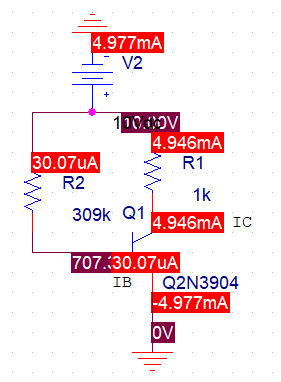
\includegraphics[width=.5\textwidth]{Figures/L3F3}
  \caption{Active Region Simulation}
  \label{fig:7}
\end{figure}

From this, we may find the $\beta$ value:

$$\beta=\frac{I_C}{I_B}$$
$$\beta=\frac{4.946}{.03007}$$
$$\boxed{\beta=164.48}$$

We may observe that this value is lower than the one obtained experimentally; however it is still a bit similar. We now move on to the saturated case:

\begin{figure}[H]
  \centering
  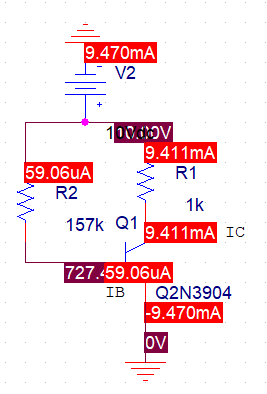
\includegraphics[width=.5\textwidth]{Figures/L3F4}
  \caption{Saturated Region Simulation}
  \label{fig:8}
\end{figure}

From this, we find:

$$\beta=\frac{9.411}{.05906}$$
$$\boxed{\beta=159.35}$$

We may observe that this value is close to the experimentally obtain value; more importantly, however, it shows that $\beta$ drops in the saturated region. Finally, we simulate the cut-off region:

\begin{figure}[H]
  \centering
  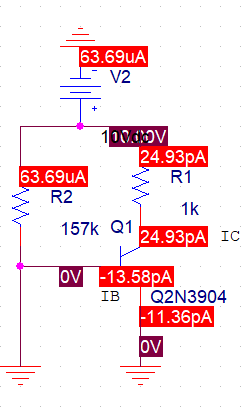
\includegraphics[width=.5\textwidth]{Figures/L3F5}
  \caption{Cut-Off Region Simulation}
  \label{fig:9}
\end{figure}

We may observe that the current flow is practically zero throughout the circuit. Given that there is nearly no current flow through the resistor $R_C$, we may obtain the same value as we obtained experimentally:

$$V_{CE}\approx 10[\si{\volt}]$$

For the touch-sensitive circuit, we may see:

\begin{figure}[H]
  \centering
  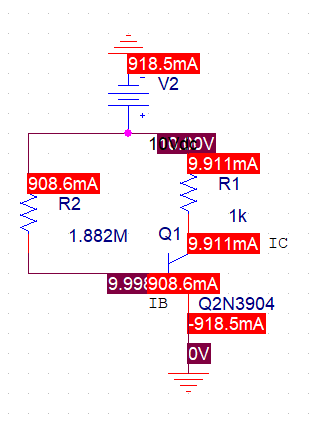
\includegraphics[width=.5\textwidth]{Figures/L3F6}
  \caption{Touch-Sensitive Equivalent Simulation}
  \label{fig:10}
\end{figure}

We may observe that the voltage drop across the resistor makes:

$$V_{CE}=10-(9.911)(1)$$
$$V_{CE}=.089[\si{\volt}]$$

Furthermore, we see that: 

$$V_{BE}= 10-(908.6)(1.882\cdot10^3)$$
$$V_{BE}= -1.71\cdot10^{6}$$

Therefore, because $V_{BE}<V_{CE}$, we may say that this BJT \underline{is in the active region}.

\subsubsection{Night Light Simulation}

We now move on to simulating the night light. We simulate once for a ``light'' case, and once for a ``dark'' case:

\begin{figure}[H]
  \centering
  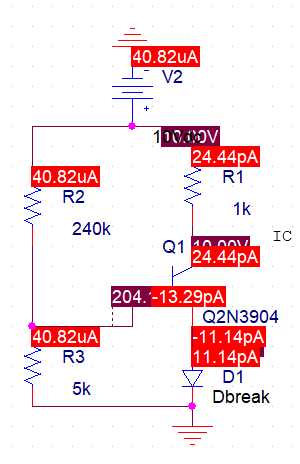
\includegraphics[width=.4\textwidth]{Figures/L3F7}
  \caption{Immediate Response ``Light'' Case}
  \label{fig:11}
\end{figure}

\begin{figure}[H]
  \centering
  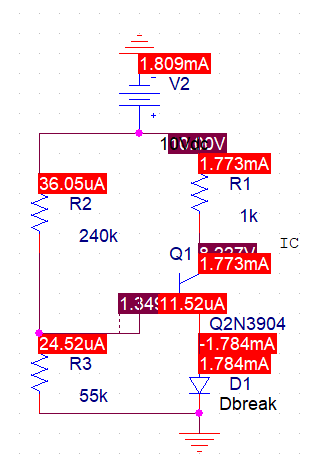
\includegraphics[width=.4\textwidth]{Figures/L3F8}
  \caption{Immediate Response ``Dark'' Case}
  \label{fig:12}
\end{figure}

We may write the gains as:

$$\beta_{light}=\frac{24.44}{-13.29}$$
$$\boxed{\beta_{light}=-1.839}$$

$$\beta_{dark}=\frac{1.773}{.01152}$$
$$\boxed{\beta_{dark}=153.91}$$

We may observe that, as intended, there is current flow through the LED when it is dark, which turns it on, and no (or, rather, limited) current flow when it is light. As we see, the circuit behaves as expected. Adding a parallel capacitor we get:

\begin{figure}[H]
  \centering
  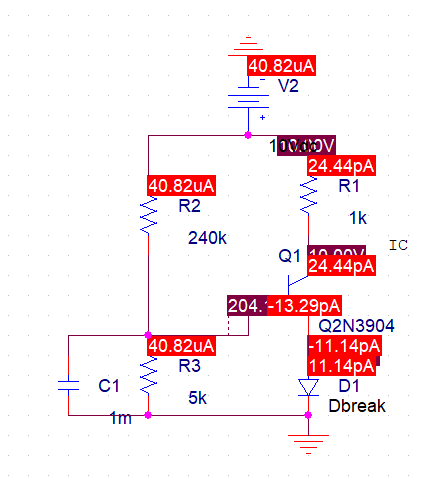
\includegraphics[width=.4\textwidth]{Figures/L3F9}
  \caption{Time-Delayed Response ``Light'' Case}
  \label{fig:13}
\end{figure}

\begin{figure}[H]
  \centering
  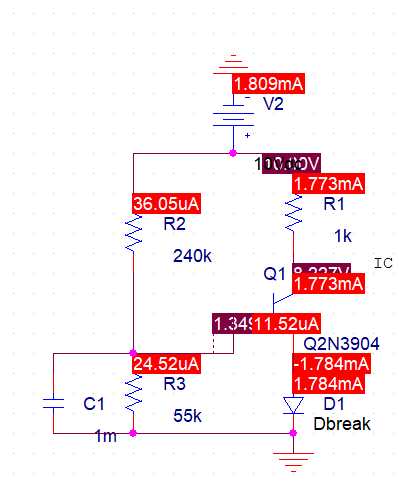
\includegraphics[width=.4\textwidth]{Figures/L3F10}
  \caption{Time-Delayed Response ``Dark'' Case}
  \label{fig:14}
\end{figure}

Since we are not running a time-sweep (transient analysis), we see that, because there is only DC input, the capacitor is treated as an open circuit, and the values remain the same. We can observe, however, that, by calculating the time constant, there is a delay for the LED to charge or discharge:

$$\tau=RC$$
$$\tau=\frac{1}{(1)(5)}$$
$$\boxed{\tau=.2[\si{\second}]}$$

This is a bit less than intended, since the measured photocell resistance values were less than expected; however, the time-delay still worked.

\section{Conclusion}

Throughout this laboratory experiment, we familiarized ourselves with the operations of bipolar junction transistors in their standard regions (active, saturated, and cut-off). We then synthesized our knowledge by constructing a touch-activated and light-sensitive circuit.

\end{document}
